\subsection{\textcolor{gray}{Detail of Design}}
The Smart Lock prototype consists of both hardware and software components, designed to provide secure, remote access control with user authentication and cloud connectivity.

\subsubsection{\textcolor{teal}{System Overview}}

Our system integrates a physical keypad-based lock with Wi-Fi-enabled remote access through a mobile application. Users can authenticate using a PIN or biometric authentication (fingerprint or facial recognition), and manage access remotely.

\begin{figure}[h]
    \centering
    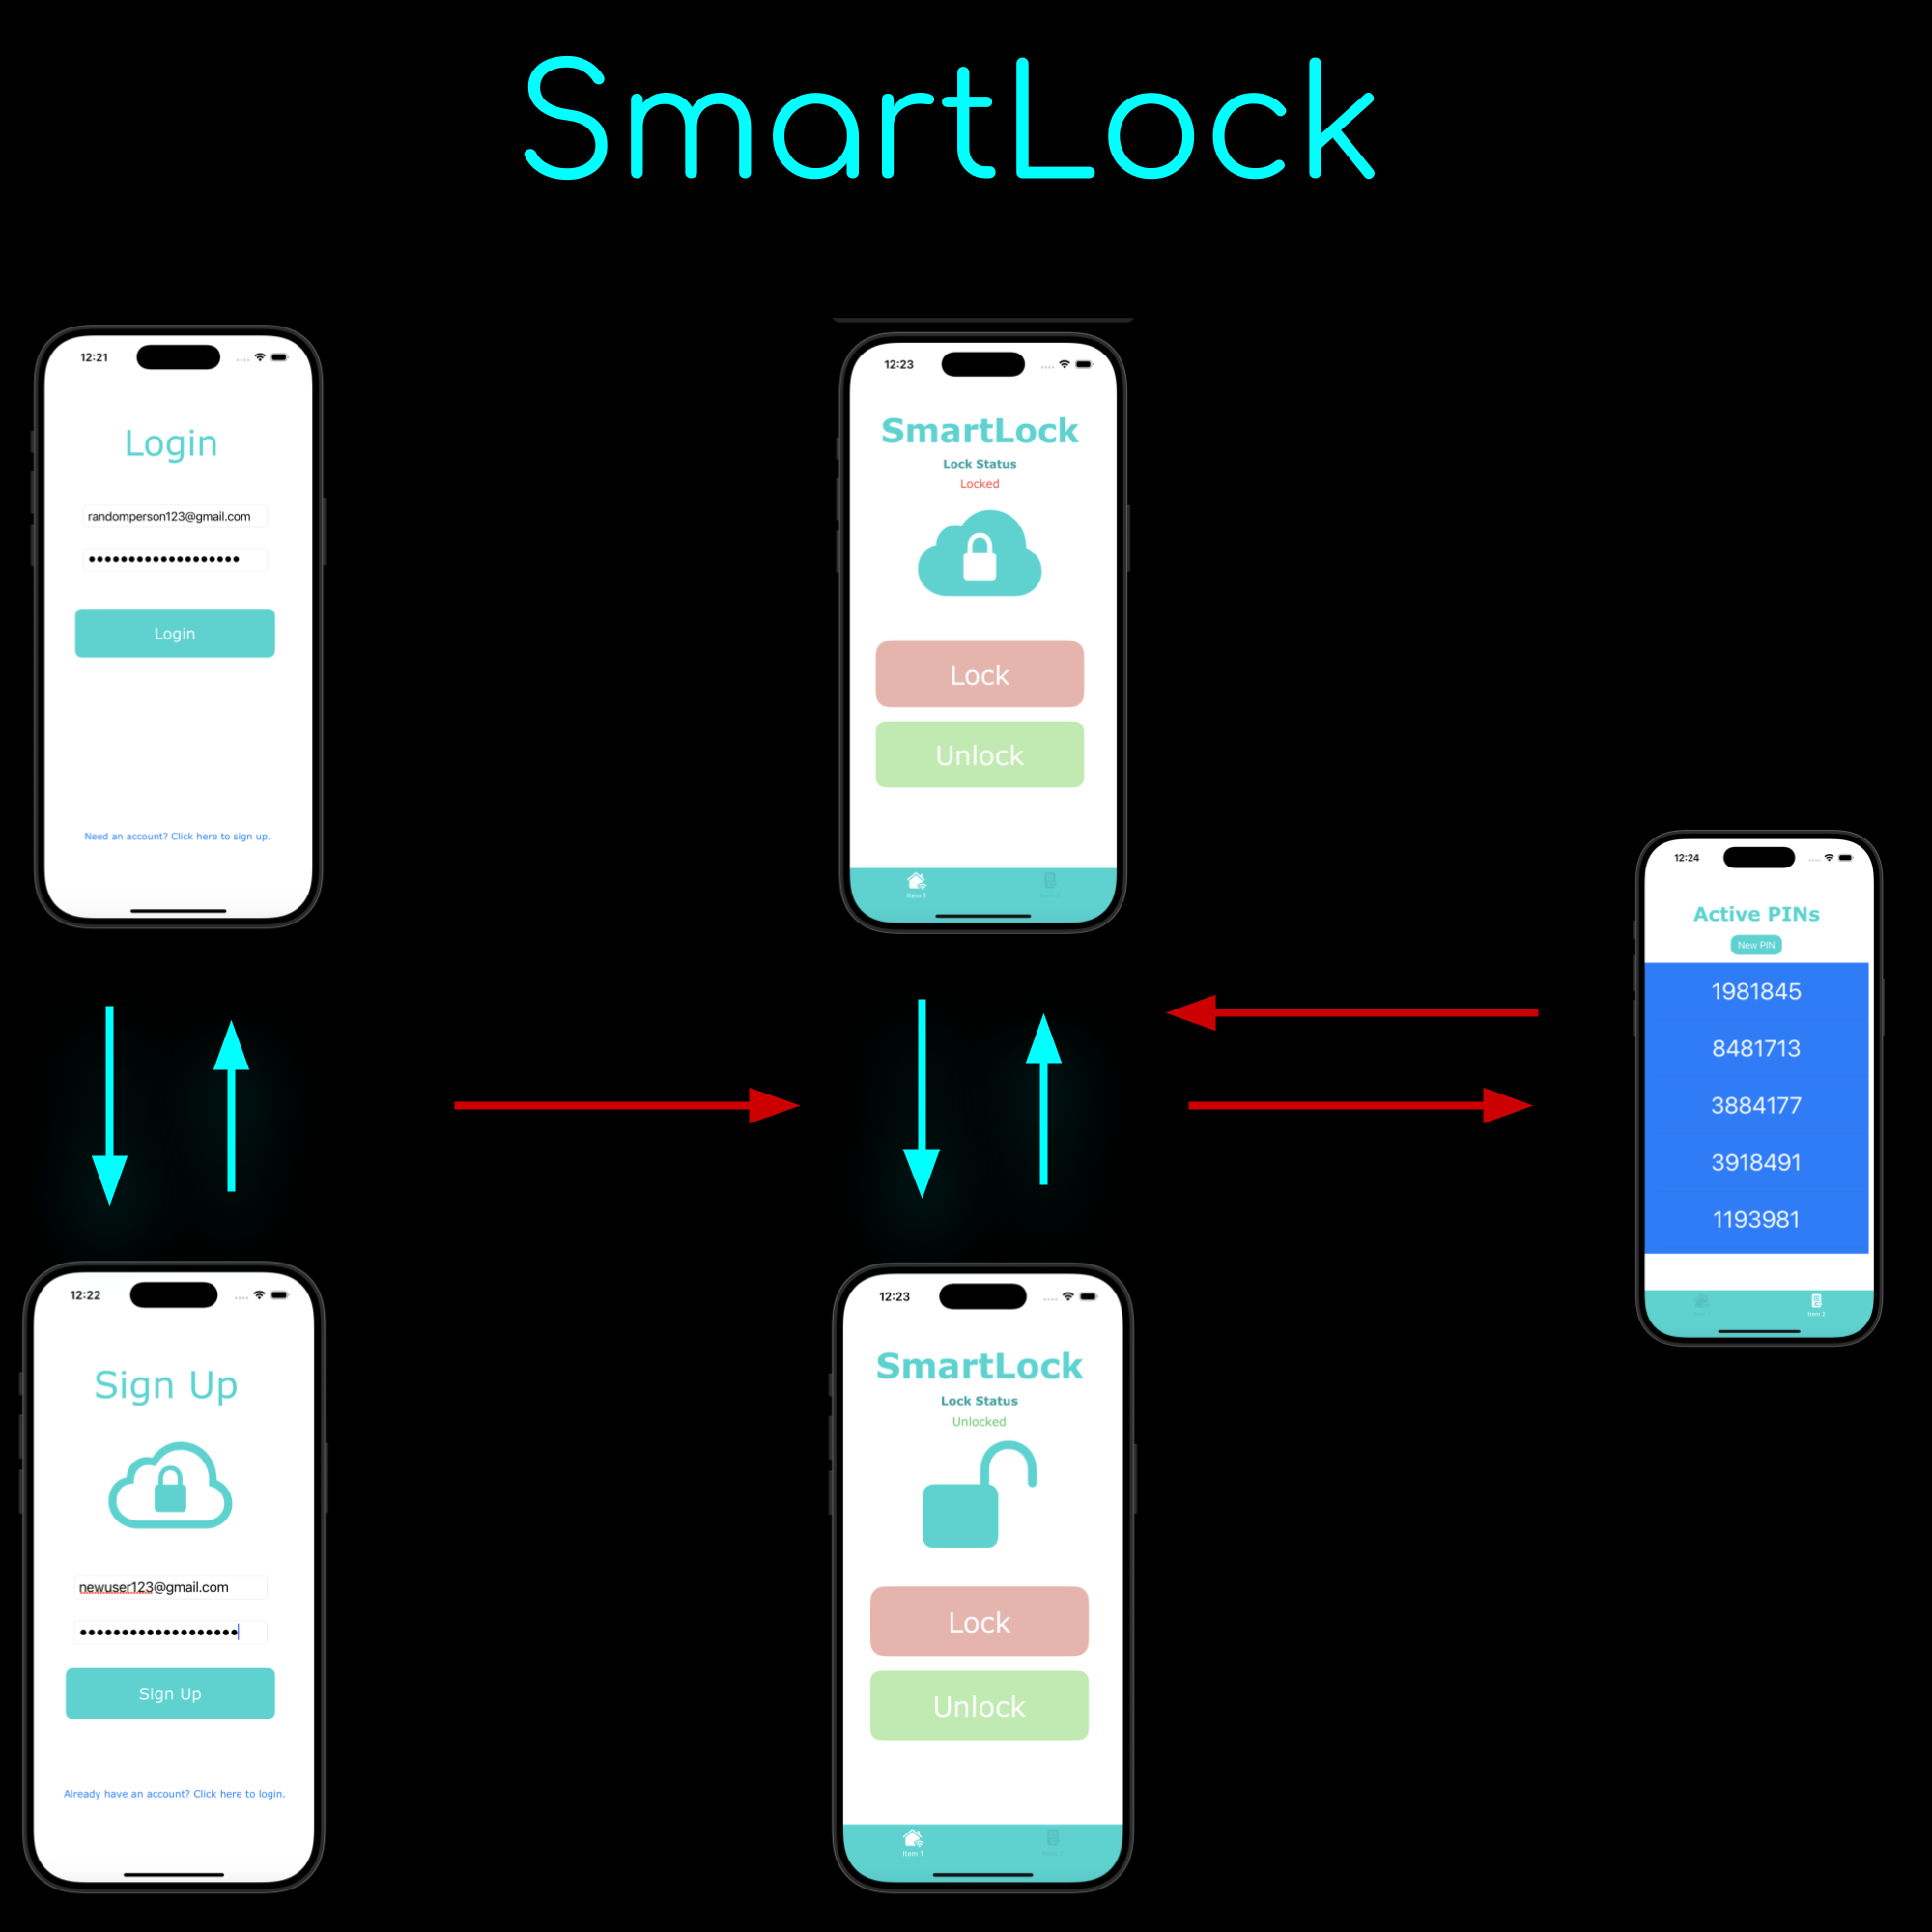
\includegraphics[width=0.65\textwidth]{./img/flowsl.png}
    \caption{Mobile App Flowchart for Smart Lock System}
\end{figure}

\begin{itemize}
    \item Users log in or create an account to access the smart lock.
    \item The main control screen provides lock/unlock buttons.
    \item Users can view and manage active PIN codes for secure access.
    \item The system communicates with a cloud database (Firestore) for real-time authentication and remote control.
\end{itemize}

\subsubsection{\textcolor{teal}{Connectivity and Cloud Integration}}

The Smart Lock is cloud-connected, enabling users to manage access remotely via a mobile app. The system:
\begin{itemize}
    \item Authenticates PIN entries locally for quick access.
    \item Processes biometric authentication for increased security.
    \item Syncs PIN codes with Firebase, allowing updates in real-time.
    \item Sends lock/unlock status to the cloud, ensuring remote monitoring.
    \item Logs user access, creating an audit trail for security.
\end{itemize}

Our cloud integration will have a many-to-many relationship with the mobile app and the lock. The mobile app will send requests to the cloud, so that there can be many users with multiple locks. Furthermore it allows the user to have control over which locks they want to unlock. To have this many-to-many relationship, we will create two different table collections. The first collection will be the user collection, which will have the user ID, email, and password. The second collection will be the lock collection, which will have the lock ID, lock name, and lock state. The user collection will have a reference to the lock collection, so that we can have multiple locks for each user. This will allow us to have a many-to-many relationship between the user and the lock. Furthermore, we are planning to use a join table to connect the two collections. The join table will have the user ID and lock ID, so that we can have multiple locks for each user and multiple users for each lock. This will allow us to have a many-to-many relationship between the user and the lock. Additionally, to add more information about each lock we can create a history collection, which will have the lock ID, user ID, and timestamp. This will allow us to keep track of which user unlocked which lock and when. This will be useful for auditing purposes and for keeping track of who has access to which locks. It will also allow us to see if there are any unauthorized access attempts to the locks. The history collection will be linked to the lock collection and the user collection, so that we can easily access the information about each lock and each user. This will allow us to have a complete picture of the access control system and will help us to identify any potential security issues. One last collection we can have is a status collection, which will have the lock ID and the status of the lock. This will allow us to keep track of the status of each lock and to see if there are any issues with the locks. The status collection will be linked to the lock collection, so that we can easily access the information about each lock. This will allow us to have a complete picture of the access control system and will help us to identify any potential security issues. We will have a diagram shown below to show the relationship between the collections and how they are connected to each other.

%% TODO: Neena import the diagram here

\subsubsection{\textcolor{teal}{Hardware Design}}

The Smart Lock hardware consists of a 3D printed casing, a keypad for PIN entry, a biometric scanner, a solenoid lock mechanism, and an ESP32-C3 microcontroller.

\begin{figure}[htbp]
    \centering
    \begin{subfigure}[b]{0.48\textwidth}
        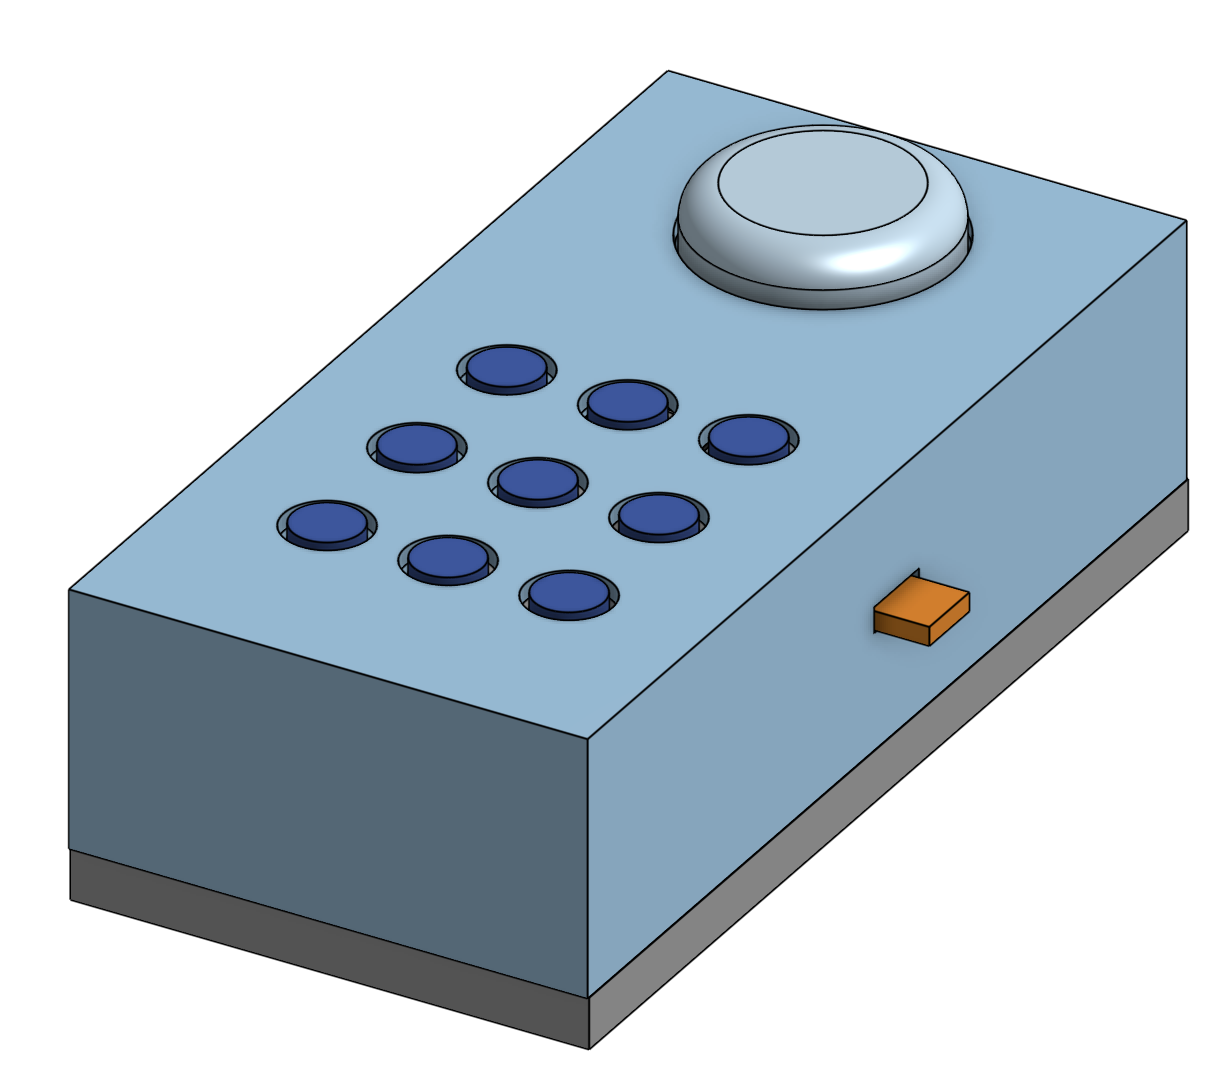
\includegraphics[width=\textwidth]{./img/isoView.png}
        \caption{Isometric View}
        \label{fig:isoView}
    \end{subfigure}
    \hfill
    \begin{subfigure}[b]{0.48\textwidth}
        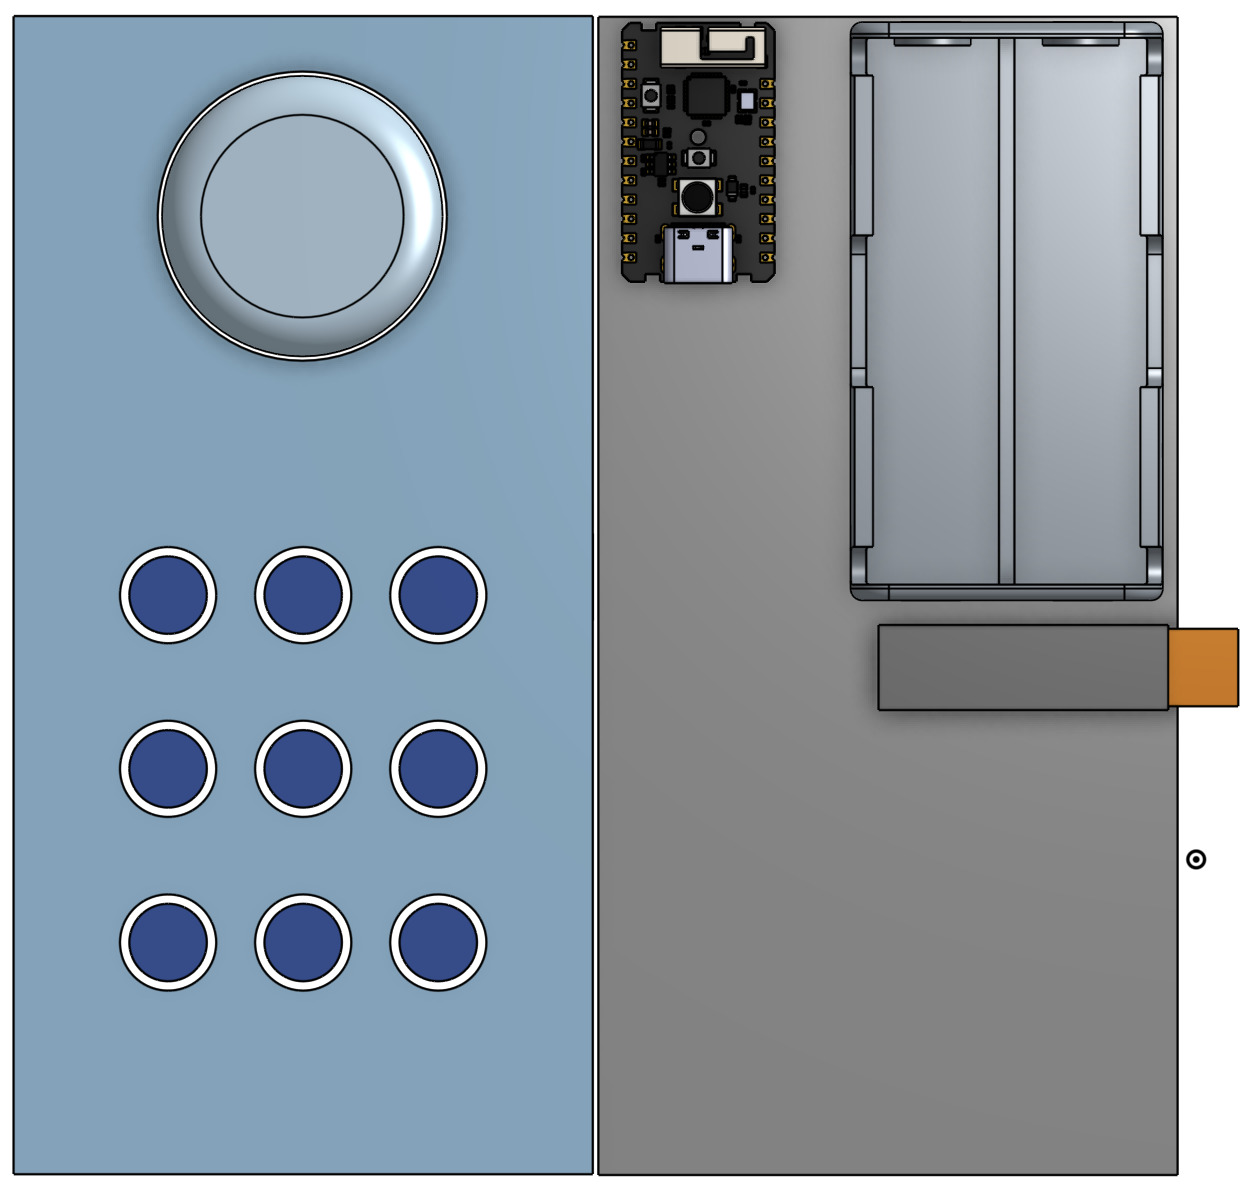
\includegraphics[width=\textwidth]{./img/topView.png}
        \caption{Top View}
        \label{fig:topView}
    \end{subfigure}
    \caption{First lock design}
\end{figure}

Here is the isometric view of the Smart Lock prototype. The top section will potentially include a biometric scanner, for fingerprint or facial recognition authentication, and a numeric keypad for PIN entry.\newline

\textbf{Key components:}
\begin{itemize}
    \item \textbf{Biometric Scanner:} Supports fingerprint or facial recognition for enhanced security
    \item \textbf{Numeric Keypad:} Users enter PIN codes as an alternative authentication method
    \item \textbf{Solenoid Lock:} Engages or disengages upon successful authentication
    \item \textbf{Microcontroller (ESP32-C3):} Handles user input, authentication, and connectivity
    \item \textbf{Rechargeable Battery:} Powers the system, ensuring reliability even in case of power outages
\end{itemize}

This design ensures compactness while maintaining modular repairability, allowing components to be easily accessed or replaced.


\subsubsection{\textcolor{teal}{Life Cycle Assessment (LCA)}}

The life cycle of the Smart Lock was analyzed to ensure sustainability and environmental responsibility. Key aspects include: \newline

\textbf{Eco-Friendly Manufacturing}
\begin{itemize}
    \item Uses locally sourced materials to minimize transportation emissions
    \item Modular design allows for easy repair and component replacement, reducing e-waste
    \item Prioritizes recyclable materials in construction
\end{itemize}

\textbf{Energy Efficiency}
\begin{itemize}
    \item Operates on a rechargeable lithium battery to extend lifespan
    \item Supports an optional solar charging module to reduce reliance on disposable batteries
\end{itemize}

\textbf{Smarter Chemistry}
\begin{itemize}
    \item Lead-free soldering eliminates hazardous materials.
    \item Arsenic- and mercury-free components ensure environmental safety.
    \item PVC-free wiring minimizes harmful plastic waste.
\end{itemize}

\textbf{End of Life Considerations}
\begin{itemize}
    \item Designed for easy disassembly, allowing parts to be recovered for recycling.
    \item Encourages users to recycle old locks through e-waste partnerships.
\end{itemize}

\textbf{Commitment to Sustainability}
\begin{itemize}
    \item Uses stainless steel casing with the option for recycled metal integration.
    \item Packaging minimizes non-recyclable plastics, favoring biodegradable materials
\end{itemize}

\begin{figure}[h]
    \centering
    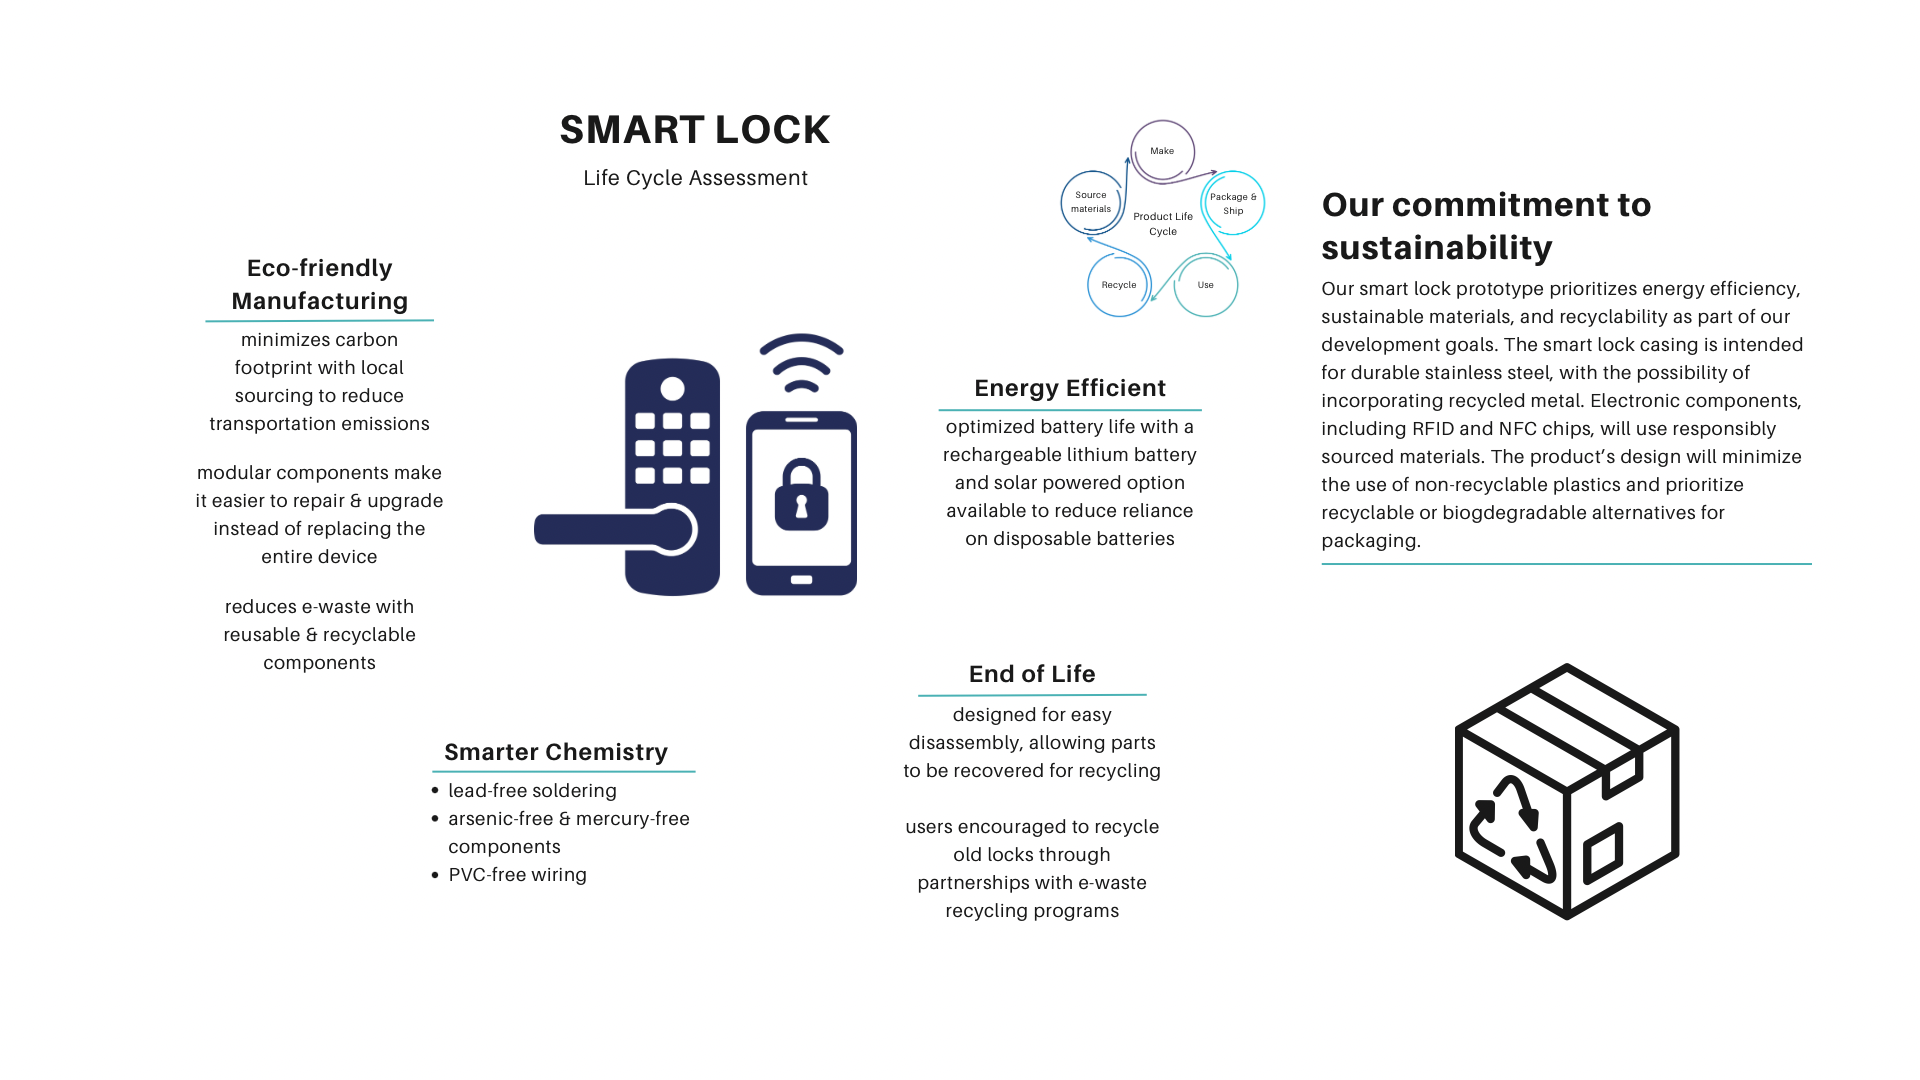
\includegraphics[width=0.8\textwidth]{./img/LifeCycleAssessment.png}
    \caption{Life Cycle Assessment of the Smart Lock}
    \label{fig:lifecycle}
\end{figure}

\noindent By integrating secure hardware, cloud-based software, and sustainable practices, the Smart Lock aims to offer a modern, environmentally responsible solution to traditional key-based access control.